\documentclass{llncs}

\usepackage{microtype}
\usepackage{amsmath,amssymb,mathtools}
\usepackage{hyperref}
\usepackage{booktabs}
\usepackage{graphicx}

\usepackage{pifont}
\newcommand{\cmark}{\ding{51}}%
\newcommand{\xmark}{\ding{55}}%

\newcommand{\etal}{et~al.\@}

\newcommand{\AppPAL}[0]{SecPAL4BYOD}

\usepackage{acronym}
\acrodef{MDM}{Mobile Device Management}

\usepackage{listings}
\lstdefinelanguage{AppPAL}{%
  morekeywords={if,inf,says,where,true,false,with,is},
  otherkeywords={can-act-as,can-say},
  sensitive=true,
  morestring=[b]',
  literate={\ inf\ }{{$\infty$}}5
}[keywords,strings]
\newcommand{\listingsize}[0]{\footnotesize}
\lstset{%
  basicstyle=\normalfont\ttfamily,%\listingsize,
  keywordstyle=\normalfont\ttfamily\slshape,%\listingsize,
  stringstyle=\normalfont\sffamily,%\listingsize,
  columns=flexible,
  mathescape,
  tabsize=2,
  showstringspaces=true,
  %numbers=left,
  frame=single,
  breaklines=true,
  numberstyle=\tiny\ttfamily\color{Gray},
  commentstyle=\ttfamily\color{Gray}
}
\newcommand{\code}[2][]{\lstinline[breaklines=true, #1]{#2}}

\usepackage{mdframed}
\newcommand{\todo}[1]{\marginpar{\begin{mdframed}[userdefinedwidth=1cm]\tiny\sffamily\raggedright #1\end{mdframed}}}

\newenvironment{policyrule}[1]{%
  \begin{mdframed}\footnotesize
      \noindent\textbf{\sffamily #1}:~\itshape%
}{%
  \end{mdframed}
}

\title{Capturing Policies for BYOD}
\author{Joseph Hallett and David Aspinall}
\institute{University of Edinburgh}
\begin{document}
\maketitle
\begin{abstract}
  % 4 Sentences
  BYOD policies are informally specified using natural language.
  Various tools and \ac{MDM} solutions can implement parts of the policies, but there isn't a means to tie the written policy to its enforcement method.
  In this paper we show how \AppPAL~can be used to capture policies for BYOD.
  We identify common BYOD idioms and delegation structures.
\end{abstract}
\section{Introduction}
\label{sec:intro}
% Describe the problem
% State my contribution
% 1 page

Employees bring their own devices to work.
In the past employees might have had a dedicated company device.
Today around 70\% of companies have a BYOD scheme~\cite{schulze_byod_2016} and, in some fields,
  85\% of staff use their personal devices to look up work-sensitive information~\cite{patel_uk_2015}.
This creates a challenge for IT departments.
They need to control access to company resources, but have limited control over the devices used to access them.

One common solution to control devices is to require users to agree to follow a policy.
These policies take the form of user agreements, written in natural language, which describe how the devices should be used and configured.
Various guides are available for companies wishing to implement a policy from governments, standards bodies, and companies seeking to advise~\cite{nicholas_r._c._guerin_security_2008,souppaya_guidelines_????,hp_byod_????,cesg_byod_2015}.
On top of user agreements companies may also use \ac{MDM} software, which can enforce some policies automatically.
The use of \ac{MDM} software does not guarantee compliance however.
One survey found over 50\% of companies with \ac{MDM} software still have un-compliant devices in their networks~\cite{mobileiron_security_labs_q4_2015}.

BYOD policies are becoming more complex and \ac{MDM} software is becoming more proficient.
There has been much work looking at developing the \ac{MDM} software to enforce aspects of BYOD policies~\cite{costantino_towards_2013,martinelli_enhancing_2016,armando_enabling_2014}.
Enforcing a policy is only part of the problem, however.
BYOD policies are specified informally using natural language, and they contain more than just access control decisions.
These policies describe trust relationships inside the company between the IT departments, users, and HR each who may be delegated to make decisions and provide rules.
Policies contain rules that require employees to acknowledge risks, and regulations.
An antivirus or \ac{MDM} program may be used to \emph{implement} part of a policy, but it is the policy which \emph{specifies} which software to use and when; there is no automatic way to check how a policy has been implemented and by what.

This paper describes a formalization of five BYOD policies using a variation of SecPAL called \AppPAL.
This has been implemented atop of AppPAL---a policy language for mobile device privacy preferences~\cite{hallett_apppal_2016}.
Using our formalization we identify the common concerns and trust relationships in these policies.
We show how \AppPAL~can be used to implement these policies, and describe precisely the different trust relationships.
\AppPAL~is an instantiation of the SecPAL authorization language~\cite{becker_secpal:_2010} for mobile device policies.
We have found, however, that it is a good fit for other policies surround the mobile ecosystem as well~\cite{hallett_specifying_2016}.
Using these papers we identify a set of standard decisions and trust relationships used in BYOD policies.
These are BYOD idioms that are capture decisions at common requirements in BYOD policies.
These give a guide for where future work implementing BYOD tools should focus their efforts to cover more aspects of policies.

\section{My Idea}
\label{sec:idea}
% 2 pages

Corporate BYOD policies are tricky to fully enforce.
Part of their policies are prescriptive:  if you configure your device in this way you will mitigate that threat.
The policies contain more than just configuration, however.
Consider this rule taken from the \emph{Security Policy for the use of handheld devices in corporate environments} by SANS~\cite{nicholas_r._c._guerin_security_2008}:

\newcommand{\textbra}[1]{\ensuremath{\left\langle \text{\sffamily #1} \right\rangle}}
\begin{policyrule}{SANS}
  Digital camera embedded on handheld devices \emph{might} be disabled in restricted environments, according to \textbra{COMPANY NAME} risk analysis.
  In sensitive facilities, information can be stolen using pictures and possibly sent using MMS or E-mail services.

  In high-security facilities such as R\&D labs or design manufacturers, camera MUST be disabled.
  Furthermore, MMS messages should be disabled as well, to prevent malicious users from sending proprietary pictures.
\end{policyrule}

To implement this policy an \ac{MDM} program, such as IBM's MaaS360 could be used~\cite{_ibm_????}.
This software supports app wrapping (where an app is recompiled to use guarded APIs), and supports security ``checkboxes'' to enable security controls and access control policies.
Using techniques like this would implement the recommendation within the rule, but the rule itself contains more than just configuration to implement.
It talks of \emph{restricted environments} decided by \emph{company risk analysis}; but how is this communicated to the device?
Does it access the list of restricted environments once, from a server?
Does it understand how the risk analysis was performed?
Can it decide on the basis of a policy if a location is restricted?
The rule also gives a security objective: \emph{prevent malicious users from sending proprietary pictures}.
The guidelines are given, however, for the specific cases of a compliant user using MMS or email.
This may not be sufficient to stop a sufficiently motivated \emph{malicious} user.

Our approach does not try to implement the policy.
Rather we attempt to capture the goals of the policy rule so that the delegations of trust, tools used, and their configuration is made explicit.
This gives us greater clarity as to which tool is being trusted to implement what policy.
It allows us to see who is being trusted to make which decisions.
It also lets us use automatic tools to uncover aspects of the policy that may be unimplemented~\cite{hallett_specifying_2016}.
Continuing with the example above, this can be expressed in \AppPAL~as:

\begin{lstlisting}
'company' says 'risk-analysis' can-say
  Location:L isHighSecurityFacility.

'company' says Device:D mustDisableIn(Location, 'camera')
  if Location isHighSecurityFacility.

'company' says Device:D mustDisableIn(Location, 'mms')
  if Location isHighSecurityFacility.

'company' says User:U hasSatisfied('proprietary pictures policy')
  if U hasDevice(D),
     D mustDisableIn(Location, 'camera'),
     D mustDisableIn(Location, 'mms'),
     Location isHighSecurityFacility.
\end{lstlisting}

When checking a policy written in a formal language we generate a certificate that shows how the policy was satisfied.
These certificates not only act as proof of how the policy was followed but also provide an audit trail.
In a company decisions may be delegated to different departments.
Knowing who made the decision in each department, and whether that was on the basis of policy or a one-off, allows auditors to see what happened when things go wrong, and builds trust that a system is working correctly.

\todo{%
  Why is the \AppPAL~better?
  Clearer, explicit, can identify problems automatically.

  Explain why I'm trying to build a schema for BYOD policies and why this is worth a paper.

  How is this falsifiable?
  Examples of policy idioms we can't express.
}



\section{The Details}
\label{sec:details}
% 5 pages

\subsection{Changes to \AppPAL}

To create \AppPAL~we instantiate SecPAL~with four kinds of facts specific to BYOD: \emph{can, has, is} and \emph{must}.
Like other SecPAL-based instantiations~\cite{becker_framework_2009,aziz_secpal4dsa:_2011} we extend the syntax of facts to support these constructs.
Internally, however, they are treated as standard predicates.

\begin{center}
  \footnotesize\sffamily
  \newcommand{\predicate}[3]{#1 \texttt{#2\textit{#3}}}
  \begin{tabular}{l l}
    \toprule
    Fact                              & Meaning                                         \\
    \midrule
    \predicate{subject}{can}{Action}  & The subject is permitted to perform the action. \\
    \predicate{subject}{has}{Action}  & The subject has performed the action.           \\
    \predicate{subject}{is}{Type}     & The subject is a member of the type.            \\
    \predicate{subject}{must}{Action} & The subject must perform the action.            \\
    \bottomrule
  \end{tabular}
\end{center}

Facts of the \emph{must}-kind represent obligations, actions that should be completed if a particular scenario presents itself.
For these facts we add a rule to ensure the obligation is performed.
This rule should be checked periodically to ensure compliance.
\begin{lstlisting}
$\langle\text{speaker}\rangle$ says $\langle\text{subject}\rangle$ hasSatisfiedObligation$\langle\text{Action}\rangle$
  if $\langle\text{subject}\rangle$ must$\langle\text{Action}\rangle$,
     $\langle\text{subject}\rangle$ has$\langle\text{Action}\rangle$.
\end{lstlisting}

When using \AppPAL~to describe policies, we also need to describe what domain each variable belongs to.
This is performed through the \emph{is}-kind facts.
\AppPAL~inherits from SecPAL (and Datalog) a safety condition that all variables in the head of an assertion must be referenced in the body.
This leads to policies which can be noisy to read.
For example in the SANS policy there is a rule that states that devices can only connect to wireless access points owned by the company.
This is written in \AppPAL~as:
\begin{lstlisting}
'company' says Device canConnectToAP(AP)
  if AP isOwnedByCompany,
     Device isDevice,
     AP isAccessPoint.
\end{lstlisting}
To simplify the presentation we allow a special sugared notation for conditionals expressing the type of a variable (\emph{variable \emph{is}Type}).
Any variable in the head of the rule of the form \texttt{\emph{Type}:Variable} is replaced by the variable and a conditional that \texttt{Variable is\emph{Type}} is added to the body.
The rule can be re-written as shown bellow hiding the typing statements.
\begin{lstlisting}
'company' says Device:D canConnectToAP(AP:X)
  if X isOwnedByCompany.
\end{lstlisting}

\subsection{BYOD Policies}
\label{ssec:byod-policies}

We analysed five different policies to find common idioms.
The first is the \emph{Security Policy Template: Use of Handheld Devices in a Corporate Environment}, published by the SANS Institute~\cite{nicholas_r._c._guerin_security_2008}.
This is a hypothetical policy published to help companies mitigate the threats to corporate assets caused by mobile devices.
Companies are expected to modify the document to suit their needs.
The policy is general; not specific to any particular industry, device, or country's legislation.
The second is taken from Healthcare Information Management System Society~\cite{healthcare_information_and_management_systems_society_mobile_2012};
  a US non-profit company trying to improve healthcare through IT.
It is relatively short but interesting because it contains concerns specific to healthcare scenarios, and is written as a contract the users are agreeing to follow.
In contrast every other policy we looked at is written as a series of rules users should follow to ensure compliance.
The policy is designed as a sample agreement for a system trying to manage personal mobile devices in a healthcare environment.
The third is taken from an British hospital trust~\cite{kennington_mobiles_2014}, and describes the BYOD scheme used in practice at the hospital.
Finally two simpler policies are taken from The University of Edinburgh~\cite{david_williamson_bring_2015} and a company specialising in emergency sirens~\cite{code3pse.org_sample_????}.
These policies are simpler than the other comprised of much more general rules and only a page or two in length.

\begin{table}\centering\footnotesize\sffamily
  \begin{tabular}{l c c c c c}
    \toprule
                             & {SANS}       & {HiMSS}     & {NHS}       & {Edinburgh} & {Sirens}    \\
    \midrule
    Number of rules          & 33           & 15          & 56          &             & 25          \\
    \AppPAL~assertions       & 71           & 21          & 58          & 10          & 39          \\
    Policy coverage          & 33 (100$\%$) & 14 (93$\%$) & 40 (71$\%$) &             & 22 (88$\%$) \\
    \midrule
    Delegations              & 23           & 5           & 33          & 2           & 13          \\
    Acknowledgement          &              &             &             &             &             \\
    Partial Acknowledgement  &              &             &             &             &             \\
    \bottomrule             \\
  \end{tabular}
  \label{tab:summary}
  \caption{Summary of the contents of each of the BYOD policies.}
\end{table}

The policies are summarised in \autoref{tab:summary}.
Each policy contains a series of \emph{rules}, which are implemented by one or more \emph{\AppPAL~assertions}.
The \emph{policy coverage} represents the number of rules that have a \AppPAL~description attached.

Not all the rules in a policy require a \AppPAL~translation.
For example rule 9.1 in the NHS policy states:
\begin{policyrule}{NHS}
  Downloading of personal apps onto a corporately issued mobile device should be avoided where possible.
  The Trust would not encourage staff members to download apps for personal use onto a corporately issued mobile device.
  All staff are reminded that they must adhere to the guidance outlined in the Social Media Policy.
\end{policyrule}
The rule does not prohibit any action, and doesn't require the staff to do anything different.
It does remind staff to be aware of a rule which we could implement with an acknowledgement; a statement that the party has acknowledged a rule.
\begin{lstlisting}
'nhs-trust' says Staff:S mustAcknowledge('avoid-installing-personal-apps').
'nhs-trust' says Staff:S mustAcknowledge('social-media-policy').
\end{lstlisting}
In this case, however, since nothing is required even an acknowledgement seems excessive.

Table~\ref{tab:byod-predicates} summarises the facts used by multiple policies.
This shows what concerns and controls and are shared between different BYOD policies.
All five of the policies make use of acknowledgements, for example.
This could be because not all the rules in a policy can be enforced through technical means, 
  or it could indicate policy authors care more that the subjects are aware of the rules than they do for rigorous enforcement.
All but the HiMMS policy have rules that include locking down a device by disabling features.
All but the Edinburgh policy have rules that look at what should happen when a device is lost,
  and have rules that require employees inform someone when something happens.
These common concerns suggest where future \ac{MDM} software should focus their efforts.

Only the NHS and SANS, the two most complex policies, describe when a device can install an app and what kinds of apps are installable.
In both policies this is predominantly limited to a delegation to the appropriate groups to authorize an app.
For example, in the SANS policy the IT-Department are responsible for deciding what apps can be installed.
\begin{policyrule}{SANS}
  The IT Department maintains lists of allowed and unauthorized applications and makes them available to users on the intranet.
  \normalfont
  \begin{lstlisting}
'company' says 'it-department' can-say App:A isInstallable.
  \end{lstlisting}
\end{policyrule}
The NHS policy, however, is significantly more complicated.
Apps have to be approved by three different groups (the Integrated Governance Committee, the Employee's manager, and the relevant group within the trust depending on where the employee works) before the trust will say that an app can be installed.
\begin{policyrule}{NHS}
  Apps for work usage must not be downloaded onto corporately issued
  mobile devices (even if approved on the NHS apps store) unless they have
  been approved through the following Trust channels:
  
  Clinical apps; at the time of writing there are no apps clinically
  approved by the Trust for use with patients~/~clients. However, if a
  member of staff believes that there are clinical apps or other
  technologies that could benefit their patients~/~clients, this should be
  discussed with the clinical lead in the first instance and ratification
  should be sought via the Care and Clinical Policies Group. A clinical
  app should not be used if it has not been approved via this group.
  
  Business apps; at the time of writing there are no business (i.e.,
  non-clinical) apps approved by the Trust for use other than those
  preloaded onto the device at the point of issue. However, if a member of
  staff believes that there are apps or other technologies that could
  benefit their non-clinical work, ratification of the app must be sought
  via the Management of Information Group (MIG). An app should not be used
  if it has not been approved via this group.

  Following approval through Care and Clinical Policies and~/~or MIG, final
  approval will be required through Integrated Governance Committee.

  Use of paid apps must be agreed in advance with the device holder's line
  manager and there should be a demonstrable benefit.
  \normalfont
  \begin{lstlisting}
'nhs-trust' says App isUsable if App hasMet('clinical-use-case').
'nhs-trust' says App isUsable if App hasMet('business-use-case').
'nhs-trust' says 'cacpg' can-say App:A hasMet('clinical-use-case').
'nhs-trust' says 'mig' can-say App:A hasMet('business-use-case').
'nhs-trust' says App isInstallable
if App hasMet('final-app-approval'),
   App isUsable.
'nhs-trust' says 'igc' can-say App hasMet('final-app-approval').
'nhs-trust' says Device canInstall(App)
  if App isInstallable,
     App isApprovedFor(Device).
'nhs-trust' says Employee:Manager can-say
  App:A isApprovedFor(Device)
  if Manager isResponsibleFor(Device).
  \end{lstlisting}
\end{policyrule}
Given that user's have privacy preferences expressible as permissions~\cite{lin_modeling_2014}, we might expect corporate policies to also express preferences about what permissions an app can have.
This does not appear to be the case, however. 
As part of selecting the apps an IT department or group may chose to use advanced instrumentation and policies~\cite{armando_enabling_2014}, or they may manually chose apps to form a curated app store as some \ac{MDM} vendors allow.
But from the perspective of the policy itself it is more important \emph{who} makes the decision rather than \emph{what} they chose, if they have an opinion at all.

\subsection{Worked Examples}

Using the NHS rules for finding approved apps (\autoref{ssec:byod-policies}) as an example, suppose an employee, \emph{Alice}, wished to get an app, \emph{\ttfamily com.microsoft.office}, approved and installed on their device.
To do so Alice would have to convince the device that \lstinline{'nhs-trust' says 'alices-phone' canInstall('com.microsoft.office').}
Alice wishes to use the app for business so in order to satisfy the policy Alice must collect the following statements:
\begin{itemize}
    \newcommand{\weitemsize}[0]{\footnotesize}
  \item {\weitemsize \lstinline{'nhs-trust' says 'com.microsoft.office' isInstallable.}\newline}
    To do this she needs a statement from the Management of Information Group that it has a business use-case, and from the Integrated Governance Comitee that it is finally approved.
    \begin{enumerate}\setcounter{enumi}{0}
      \item {\weitemsize \lstinline{'mig' says 'com.microsoft.office' hasMet('business-use-case').}}
      \item {\weitemsize \lstinline{'igc' says 'com.microsoft.office' hasMet('final-app-approval').}}
    \end{enumerate}
  \item {\weitemsize \lstinline{'nhs-trust' says 'com.microsoft.office' isApprovedFor('alices-device').}}
    To get this she needs a statement from the manager responsible for Alice's device (\emph{Bob}) approving the app.
    \begin{enumerate}\setcounter{enumi}{2}
      \item {\weitemsize \lstinline{'bob' says 'com.microsoft.office' isApprovedFor('alices-device').}}
      \item {\weitemsize \lstinline{'nhs-trust' says 'bob' isResponsibleFor('alices-device').}}
    \end{enumerate}
  \item Additionally she needs the following typing statements.
    \begin{enumerate}\setcounter{enumi}{4}
      \item {\weitemsize \lstinline{'nhs-trust' says 'com.microsoft.office' isApp.}} \label{item:isapp}
      \item {\weitemsize \lstinline{'nhs-trust' says 'bob' isEmployee.}}
    \end{enumerate}
\end{itemize}

Alice obtains the statements by contacting each of the speakers. 
Each may either give her the statement she needs or may give her additional rules.
For example the MIG and IGC may be happy to state their assertions (after a review).
When checking if the app is an App in \autoref{item:isapp}, the NHS trust may be instead inclined to delegate further.
They could reply that if the App is in the Google Play store then they're convinced it is an app.
Alice would then have to obtain additional statements if she wanted to prove this statement.
As with SecPAL, all assertions should be accompanied by a signature from their speaker proving they said the assertion.
Alternatively the speaker could refuse to give the statement, either because they don't believe it to be true, or they cannot give an answer.
In this case Alice would have to look for an alternative means to prove the statement or accept that they cannot install the app.

Once all the statements have been collected into an \emph{assertion context}.
Alice can use a SecPAL inference tool (such as AppPAL~\footnote{https://github.com/apppal/libapppal}) to check the policy has been satisfied.

\begin{table}\centering\footnotesize
  \newcommand{\angledtitle}[1]{\rlap{\rotatebox{45}{#1}}\hspace{1em}}
  \sffamily
  \begin{tabular}{l c c c c c p{0.45\linewidth} }
    \toprule
    Predicate                                   & \angledtitle{Sirens}   & \angledtitle{Edinburgh} & \angledtitle{HiMMS} & \angledtitle{NHS} & \angledtitle{SANS}
    & Description                                                                          \\
    \midrule
    Device \texttt{canBackupTo}(Server)         &                        & \cmark                  & \cmark              &                   &
    & Says the device may send backups to a server.                                        \\
    Device \texttt{canCall}(Number)             &                        &                         &                     & \cmark            & \cmark
    & Says the telephone numbers a device can call.                                        \\
    Device \texttt{canConnectToAP}(AP)          &                        &                         & \cmark              &                   & \cmark
    & Says a device may associate with an access point.                                    \\
    Device \texttt{canConnectToNetwork}(Subnet) & \cmark                 &                         &                     &                   & \cmark
    & Says the device may connect to a network, for example computers all within a subnet. \\
    Device \texttt{canConnectToServer}(IP)      &                        &                         &                     & \cmark            & \cmark
    & Says the subject (a device) can connect to a given server (identified by a URL).    \\
    Device \texttt{canInstall}(App)             &                        &                         &                     & \cmark            & \cmark
    & Says the device may install an app.                                                  \\
    User \texttt{canMonitor}(Device)            & \cmark                 &                         &                     & \cmark            & \cmark
    & Says the subject (a user) can monitor and unlock a device.                           \\
    Device \texttt{canStore}(File)              &                        &                         & \cmark              &                   & \cmark
    & Says a device may store some data in permanent (non-transient) storage.              \\
    User \texttt{canUse}(Device)                &                        &                         &                     & \cmark            & \cmark
    & Says a user may use a device.                                                        \\
    User \texttt{hasAcknowledged}(Policy)       & \cmark                 & \cmark                  & \cmark              & \cmark            & \cmark
    & Says an individual has acknowledged a policy.                                        \\
    Device \texttt{hasFeature}(Feature)         &                        & \cmark                  &                     & \cmark            &
    & Says a device has a feature enabled.                                                 \\
    Something \texttt{hasMet}(Policy)           &                        & \cmark                  &                     & \cmark            & \cmark
    & Says a something has met a given set of requirements.                                \\
    Device \texttt{isActivated}                 &                        &                         & \cmark              & \cmark            & \cmark
    & Specifies a device has been activated for BYOD usage.                                \\
    App \texttt{isApp}                          & \cmark                 &                         & \cmark              & \cmark            & \cmark
    & Specifies an app.                                                                    \\
    Something \texttt{isApproved}               &                        &                         & \cmark              &                   & \cmark
    & Specifies that something has been vetted and approved of.                            \\
    Data \texttt{isData}                        & \cmark                 &                         &                     &                   & \cmark
    & Specifies data.                                                                      \\
    Device \texttt{isDevice}                    & \cmark                 & \cmark                  & \cmark              & \cmark            & \cmark
    & Specifies a device.                                                                  \\
    User \texttt{isEmployee}                    & \cmark                 & \cmark                  &                     & \cmark            & \cmark
    & Specifies that someone is an employee.                                               \\
    Device \texttt{isEncrypted}                 &                        & \cmark                  &                     & \cmark            & \cmark
    & Specifies a device is encrypted.                                                     \\
    Feature \texttt{isFeature}                  & \cmark                 &                         &                     &                   & \cmark
    & Specifies a feature.                                                                 \\
    App \texttt{isInstallable}                  &                        &                         &                     & \cmark            & \cmark
    & Specifies an app is installable.                                                     \\
    Device \texttt{isLost}                      & \cmark                 &                         & \cmark              & \cmark            & \cmark
    & Specifies a device is missing.                                                       \\
    Device \texttt{isOwnedBy}(User)             & \cmark                 & \cmark                  & \cmark              & \cmark            & \cmark
    & Specifies something's owner.                                                         \\
    File \texttt{isSecurityLevel}(Level)        &                        &                         & \cmark              &                   & \cmark
    & Specifies some data as having business sensitive information.                        \\
    Something \texttt{isString}                 & \cmark                 &                         &                     & \cmark            &
    & Specifies a string.                                                                  \\
    Number \texttt{isTelephoneNumber}           &                        &                         &                     & \cmark            & \cmark
    & Specifies a telephone number.                                                        \\
    User \texttt{mustAcknowledged}(Policy)      & \cmark                 & \cmark                  & \cmark              & \cmark            & \cmark
    & Requires the user to acknowledge a  policy.                                          \\
    Device \texttt{mustDisable}(Feature)        & \cmark                 & \cmark                  &                     & \cmark            & \cmark
    & Forces the disablement of a feature (or a device).                                   \\
    User \texttt{mustInform}(User, Something)   & \cmark                 &                         & \cmark              & \cmark            & \cmark
    & Forces someone to disclose something to someone.                                     \\
    Device \texttt{mustWipe}                    & \cmark                 &                         & \cmark              & \cmark            &
    & Forces a device to be erased.                                                        \\
    \bottomrule
  \end{tabular}
  \caption{Summary of \AppPAL~facts used in multiple BYOD policies.}
  \label{tab:byod-predicates}
\end{table}

\subsection{BYOD Idioms}
\todo{Describe common idioms and patterns found in each of the policies.  Check the earlier draft for some starting work}

\subsubsection{Acknowledgement}

All of the policies looked at require their subjects to be aware and acknowledge certain rules or policies, 
  or that the company may perform certain actions.
For example the NHS and HiMSS policies state that the company will wipe devices remotely to protect confidential information if the device is lost.
Alongside these rules both policies also state that if an employee has personal information on the device then this will be lost also.
The employee is required to be aware of this, and in the case of the HiMSS policy, agree to hold the company harmless for the loss.

\begin{center}
  \noindent
  %\begin{minipage}{0.49\linewidth}
    \begin{policyrule}{HiMSS}
      I agree to hold XYZ Health System harmless for any loss relating to the
      administration of PDA/Smartphone connectivity to XYZ Health System systems
      including, but not limited to, loss of personal information stored on a
      PDA/Smartphone due to data deletion done to protect sensitive information
      related to XYZ Health System, its patients, members or partners.
      \normalfont
      \begin{lstlisting}
'xyz-health-system' says 'user' mustAcknowledged('data-loss-policy').
      \end{lstlisting}
    \end{policyrule}
  %\end{minipage}
  %\begin{minipage}{0.49\linewidth}
    \begin{policyrule}{NHS}
      Individuals who have personal data of any kind stored on a corporately
      issued mobile device must be aware that in the event of loss of the device
      the above data wipe will include removal of all personal data.
      \normalfont
      \begin{lstlisting}
'nhs-trust' says Staff:S can-say
  S hasAcknowledged('data-loss-policy').
'nhs-trust' says Staff:S mustAcknowledged('data-loss-policy').
      \end{lstlisting}
    \end{policyrule}   
  %\end{minipage}
\end{center}

Both the SANS and the siren-company policies use acknowledgements to link to other sets of rules that employees should be aware of.
These policies aren't further specified, and in the case of an acceptable use policy may be hard to enforce automatically.

\begin{policyrule}{SANS}
  Users MUST agree to the email security/acceptable use policy and eventually to the eCommerce security policy.
  \begin{lstlisting}
'company' says Employee:U mustAcknowledged('email-security'). 
'company' says Employee:U mustAcknowledged('acceptable-use'). 
'company' says Employee:U mustAcknowledged('ecommerce-security').
  \end{lstlisting}
\end{policyrule}
\begin{policyrule}{Sirens}
  The employee is expected to use his or her devices in an ethical manner at all times and adhere to the company's acceptable use policy.
  \begin{lstlisting}
'department' says Employee:E mustAcknowledged('acceptable-use').
  \end{lstlisting}
\end{policyrule}

\todo{Provide a template for what kinds of policy should be implemented like this and template \AppPAL.}

\subsection{Delegation and Roles within Policies}

\AppPAL~requires all assertions be made by an explicit speaker.
When translating the policies the author of the policy is generally used as the speaker of the rule (\autoref{tab:principals}),
  with the exception of the HiMSS policy that is written as a contract the user is agreeing to.
All the policies delegate also describe other entities that might also make assertions.
With \AppPAL~policies any speaker can delegate a decision to another speaker (with restrictions on re-delegation).
This might be to a user to acknowledge a policy, or it might be to other groups in the company who are responsible for certain decisions.

In all of the policies we looked at the majority of the decisions are made by three speakers: 
  the company, the IT-department, and the users or employees.
All of the policies also delegate to a user (apart from HiMSS where the user is the primary speaker).
The user is typically responsible for providing information, such as agreements to policies, reporting devices missing, and updating passcodes.

The Sirens, SANS and NHS policy each describe an IT-department who are delegated to make some decisions.
The HiMSS policy also describes an \emph{xyz-health-system}, who act similarly to an IT-department.
These decisions are more varied and can overlap with the responsibilities of the company.
In the NHS and SANS policies the IT department is responsible for maintaining lists of activated devices.
In the Sirens and SANS policies the IT department maintains a list of what is installable on a device or not.

\begin{table}\centering\footnotesize
  \begin{tabular}{l l}
    \toprule
    Policy      & Primary Speaker           \\
    \midrule
    {SANS}      & \emph{company}            \\
    {HiMSS}     & \emph{user}               \\
    {NHS}       & \emph{nhs-trust}          \\
    {Edinburgh} & \emph{records-management} \\
    {Sirens}    & \emph{department}         \\
    \bottomrule
  \end{tabular}
  \label{tab:principals}
  \caption{Principal Speakers from each of the policies examined.}
\end{table}

\section{Comparison with Existing MDM Software}

To evaluate \AppPAL~we compare it to existing MDM~tools: IBM's MaaS360, MobileIron, and VMWare's AirWatch; each leading MDM packages~\cite{rob_smith_magic_2016}.
We used the Android versions of each of these tools as they all supported Android.
Each of these tools support enforcing and checking compliance policies. 
They do not, however, use policy languages to specify policies; rather they supply canned policies and rules that admins can tweak.

Acknowledgements form a large portion of the BYOD policies we looked at but are not addressed by the MDM software at all.
MaaS360 can associate users with devices, and can assign them into groups.
It can distribute documents (which could include written policies) but there is currently no means to track what policies a user has agreed to or should be agreeing to.
Administrators could add user's who've acknowledged a policy to a group
One might imagine that users who have acknowledged some additional rules might be added to additional groups with stricter or more relaxed policies, but this is a semi-manual process for an administrator to set up and manage.
In contrast \AppPAL{} is more flexible. 
It allows a user to state which policies they have acknowledged, and for policies to delegate the acknowledgement of the policy to the user.
We can require that a user must acknowledge certain policies if they meet certain criteria;
and once the assertion has been made it can be imported wherever and used in making other decisions.

This lack of flexibility extends to trying to compose policies. 
Consider the following rule taken from the SANS policy:
\begin{policyrule}{SANS}
Any non business-owned (that, is private) device must be able to connect to Company network MUST first be approved by technical personnel such as those from the Company IT department or desktop support.
If allowed, privately-owned handheld devices MUST comply with this security policy and MUST be inventoried along with corporate handhelds, but identified as private. This is in order to prevent theft of corporate data with unmanaged handhelds (i.e. owner of device is not identified).
\end{policyrule}
Implementing this in an MDM solution such as MaaS360 administrators can mark some devices as being privately owned.
A group could be set up for approved privately-owned devices.
MaaS360 allows the creation of groups based on search criteria, (\autoref{fig:maas360search}), though the groups are not dynamic\footnote{The search would need to be re-run when new devices were added or a device's status changed.}.
Technical personnel could be given an administrator login to the MDM software to add devices to this group periodically, and could pass them along for inventorying.
Again the management of \emph{who} is \emph{technical personnel} is effectively manual, with optional searches to define groups.
Once we find those devices that we should allow to connect to a network we can add an access control rule to as well as enforcing the general security policy on.

\begin{lstlisting}
'company' says Device:D canConnectTo(Network:N)
  if N isCompanyOwned,
     D isPrivatelyOwned,
     D isApproved,
     D hasMet('security-policy').

'company' says 'technical-personnel' can-say
  Device:D isApproved.

'company' says 'it-department' can-act-as 'technical-personnel'.
'company' says' 'desktop-support' can-act-as 'technical-personnel'.
\end{lstlisting}

In contrast using \AppPAL~all relationships are specified by the policy.
We are free to use conformance to one policy as a conditional for applying a second.
Roles such as being \emph{technical personnel} can be given to users holding other roles without requiring manual intervention.
Furthermore the \AppPAL~rule is presented in much the same form as the rule in the policy document:  device can do action if checks are satisfied.




\begin{figure}\centering
  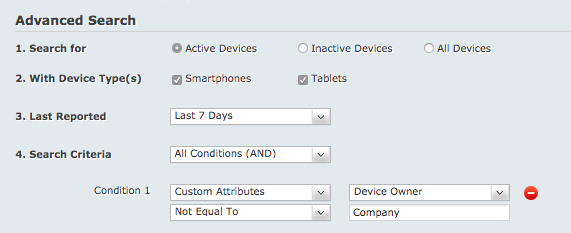
\includegraphics[width=\linewidth]{figures/maas-groupsearch.png}
  \caption{MaaS360's search interface for devices.}
  \label{fig:maas360search}
\end{figure}

\section{Related Work}
\label{sec:related}
% 1-2 pages

Companies have very little visibility into how their policies are implemented.
Morrow notes that \emph{``particularly with the BYOD trend IT professionals don't know if anti-virus software is installed or if it it's current''}~\cite{morrow_byod_2012}.
Even when devices have means to implement policies correctly it is difficult to ensure devices are properly configured when they are not corporately owned~\cite{tokuyoshi_security_2013}.
Our work aims to address these problem directly: by using formal languages we can link the policy to the implementation.

Armando~\etal~developed BYODroid as a tool for enforcing BYOD policies through a secure marketplace~\cite{armando_enabling_2014}.
Their tool allows companies to distribute a secure app~store where through a combination of static and dynamic tools they can verify that apps follow fine-grained permission policies.
Their policies are low level, based on ConSpec~\cite{aktug_conspec_2008}, allowing checks based on the JVM state.
Using their tool they implemented parts of a policy relating to personal networks, and data management for the NATO Communications and Information Agency~\cite{armando_developing_2016}.
Their work shows how parts of a BYOD policy can be checked for and enforced using tools.
A \AppPAL~policy might use BYODroid to ensure that a parts of a policy are enforced (as well as other tools for other parts).
\AppPAL~makes explicit how the natural language policy is implemented and by which tools.

Costantino~\etal~created a role-based access control scheme for BYOD devices that allowed a company to verify the devices within their network and what servers and services they had access to~\cite{costantino_towards_2013}. The scheme relied on devices having a TPM however to ensure policy violations were reported.

Other work has looked at using app wrapping to enforce more general policies.
Tools, such as Dr.~Android and Mr.~Hyde~\cite{jeon_dr._2012} and Aurasium~\cite{xu_aurasium:_2012}, have suggested app wrapping as a possible way to enforce policies.
This has the advantage that the device's underlying OS needn't be modified as the apps can be modified at the source code level.
Many commercial \ac{MDM} solutions offer app-wrapping as a feature~\cite{_ibm_????,_app_????}, however app wrapping alone without additional analysis is insufficient to enforce policies effectively~\cite{hao_effectiveness_2013}.



\section{Conclusions}
\label{sec:conclusions}
% 1/2 page



\bibliography{paper}{}
\bibliographystyle{plain}
\end{document}
